\documentclass[fontsize=12pt,a4paper]{scrartcl}
 
% Das Prozent\item Zeichen leitet einen Kommentar ein,
% es hilft ebenso, im Text Leerzeichen zu unterbinden.
 
% fontsize=12pt  Schriftgroesse in 10, 11 oder 12 Punkt
% a4paper        Papierformat ist hier A4
% landscape      Querformat wird natürlich unterstützt ;\item )
% parskip        Absatzabstand anstatt Einzüge
% draft          Der Entwurfsmodus deckt Schwächen auf
% {scrartcl}     Die Dokumentenklasse book, report, article
%                oder fürs deutsche scrbook, scrreprt, scrartcl
 
%\usepackage[ngerman]{babel} % Deutsche Sprachanpassungen
\usepackage[T1]{fontenc}    % Silbentrennung bei Sonderzeichen
\usepackage[latin1]{inputenc} % Direkte Angabe von Umlauten im Dokument.
                            % Wenn Sie an einem Mac sitzen,verwenden
                            % Sie ggf. „macce“ anstatt „utf8“.
 
\usepackage{textcomp}       % Zusätzliche Symbolzeichen
\usepackage{siunitx}
\usepackage{amsmath}
\usepackage{graphicx}
\usepackage{listings}
\lstset{tabsize=4, showspaces=false}


\title{Machine Learning SS2013}
\subtitle{Ulrike von Luxburg \\ Assignment 10}
\author{Arne Schr�der \and Falk Oswald \and Angel Bakardzhiev}
 
\date{\today}               % \today setzt das heutige Datum
 
\begin{document}
\maketitle                  % Titelei erzeugen
% \tableofcontents            % Inhaltsverzeichnis anlegen

\section*{Exercise 1: Data processing chain}

\subsection*{Regression}
We performed regression on the cancer dataset.
We compared linear regression with polinomial regression. Both seem to work pretty well, as they have both only a few miss-classifications.

    \begin{figure}[h!]
        \centering
        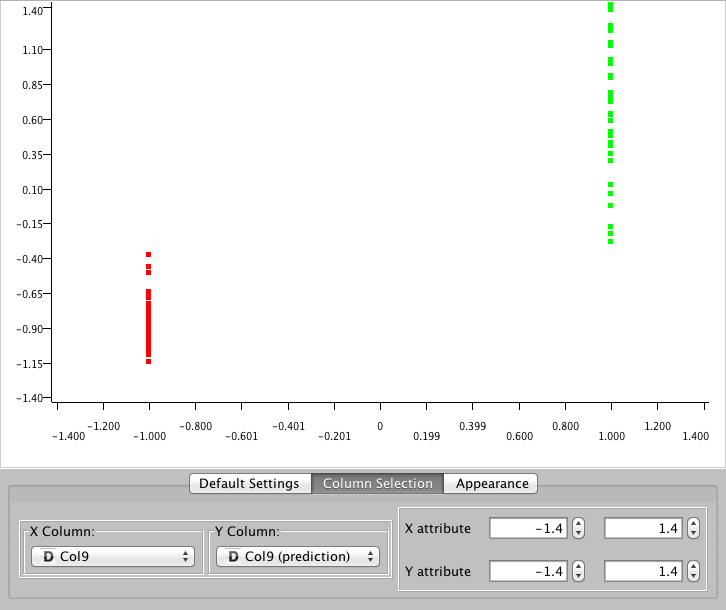
\includegraphics[width=0.9\textwidth]{reg_lin_cancer.PNG}
        \caption{Linear regression result. Y axis are the prediction results, X axis the labels.}
    \end{figure}

    \begin{figure}[h!]
        \centering
        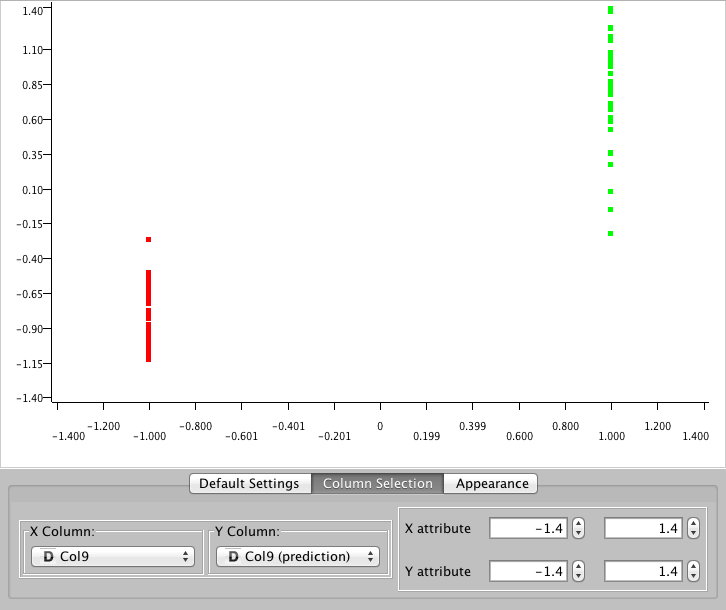
\includegraphics[width=0.9\textwidth]{reg_poly_cancer.PNG}
        \caption{Polynomial regression result. Y axis are the prediction results, X axis the labels.}
    \end{figure}
    
However, the polynomial regression (with degree 2) works slighty better as there are even less missclassifications.	
\end{document}
